\documentclass[12pt]{article}

\usepackage{graphicx}
\usepackage[margin=1.25in]{geometry}

\newcommand{\names}{Avram Twitchell, Angel Dhungana}
\newcommand{\class}{Data Mining}

\title{Determining Musical Influences with Clustering}
\author{\names \\
        \class }
        
% Requirements:
% 1.  Provide a succinct title for your project (and your names!).
%       This is part of 4 pages/student.
%       Your poster must have the same title.
% 2.  Explain the problem and motivation.
%       If you prepared a thorough proposal and intermediate report,
%       then you may be able to borrow some material from there.
% 3.  Explain what data you explored? 
%       Where did it come from, how did you process it? 
%       If you simulated toscale the experiments, how did this work? 
%       If your data collection report was thorough, you can likelyreuse much of this material.
% 4.  What is the key idea your project is built upon?
%       If there is no interesting ideas,  I will be a little disappointed. 
%       This should describe the rational behind and what you were hoping to discover
%       about the different approaches you are comparing,
%       or what extension you are proposing to a existing technique, 
%       or how you are applying a technique to a dataset where it has not been explored before.
%       State this clearly in the beginning; try to make me excited to read the remainder
%       of your report to find out how your idea played out!
% 5.  Explain what you did.
%       Did you prove something?  
%       Did you implement something?
%       Did you compare several things?
%       Did you extend something?
% 6.  Explain what you learned.
%       This is often greatly aided through charts of experiments.
%       But you shouldalso include what lessons you came away with in words; just charts or mathematics is insufficient.

\begin{document}
    \begingroup
        \let\newpage\relax%
        \maketitle
    \endgroup

    \section{Introduction}
        Spanish artist Pablo Picasso allegedly once said "Good artists copy, great artists steal."
The quote becomes all the more shocking considering that Picasso is one of the most
well-regarded artists ever, and invented an entirely new style of painting.
But artists across all mediums--painters, musicians, writers--
do not create their work in a vacuum.
They get inspired by, collaborate with, respond to, and even copy or steal from other artists.
Artists are often frank in their inspirations as well, citing other artists as influences.

The motivation of our project is to explore how artists influence each other.
We are doing this in the context of contemporary music.
In music, there are commonly accepted narratives as to how certain artists or genres
influence each other.
Human listeners can often identify an artist's influences by common
characteristics between the artists, such as instrumentation, tempo, lyrics, song structure,
or beats.

We want to see if we can identify and quantify these influences and similarities
between artists, genres, and years.
Specifically, we want to see if we can identify "progenitor" songs or artists
that had a great impact on future songs.
The idea is that, for example with Rock music, presumably an artist such as The Beatles
will have an outsized impact on subsequent Rock artists.
If we consider The Beatles as a "progenitor" group,
can we use characteristics from their songs to link to those influenced by their music?
Or, put in another way, can we identify artists who "steal" from The Beatles?

    \section{Data}
        To explore these relationships, we used the Million Song Dataset.
This is a freely-available dataset consists of features and metadata on one million contemporary songs,
produced by The Echo Nest.
While the dataset does not include actual audio,
its features include a large variety of measurements.

Many features come from analyzing segments of a song:
each song is divided into many segments, and measurements are made on each segment.
These measurements include features such as loudness or pitch.
Other features are more summary variables on the entire song, such as "danceability."
For the purposes of our analysis, we focused on the segmented features,
and did not use any "summary" variables.
We did this to see if we could identify aural commonalities within the songs themselves,
rather than broad measurements of the entire song.

\begin{figure*}[ht]
    \centering
    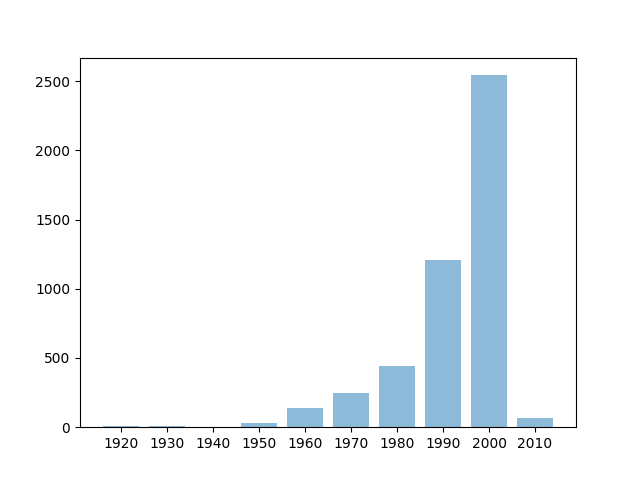
\includegraphics[width=.9\textwidth]{decade_counts}
    \caption{Data Distribution across Decades}
    \label{fig:decade}
\end{figure*}

We preprocessed these segmented measures by using the idea of k-grams.
That is, for a measure like "loudness", we took $k$ consecutive measures of loudness
in a song, and 
count that particular sequence of loudness as a unique variable.
We then represent each song as a count of the occurrences of each sequence for every variable.
Thus our preprocessed dataset is a sparse matrix of counts for each unique variable.

It should be noted that while our dataset is titled the Million Song Dataset,
much of this data is no longer available through the means listed at the project website.
Thus we ran our experiments on a 1\% subset of the data (totalling 10,000 songs).
While this is unfortunate, we feel that our conclusions in this report likely apply to
the larger dataset as well.

    \section{Methodology}
        \subsection{Lloyd's Extension}

To identify similarities between songs, we extended the Lloyd's clustering algorithm.
Since we are focusing on finding progenitors, we wanted to adapt Lloyd's algorithm
in a way that would place cluster centers around the oldest songs in the dataset.
That way, we could attempt cluster all songs--both old and newer songs--
around characteristics of older songs.

Normal Lloyd's clustering sets each cluster's center as the average of all data points in the cluster.
Our extension only looks at the oldest songs (by release year) in each cluster,
and sets the center as the average of those oldest songs.

One parameter to consider with our clustering extension is how do we define the "oldest" songs.
For example, we could consider it as the oldest 1, 5, or 10\% of the songs in a cluster.
However, for this report, we defined this as the earliest year of release in a cluster.
All songs that were released that year in the cluster are averaged to be set as the center.

\subsection{Expectations}

As far as expectations for results, we hope to see good separation between genres, and perhaps between artists as well.
This is because if our "musical lineage" hypothesis is correct,
we would expect to see very distinct genres in separate clusters with their "ancestors".
We don't expect to see good separation across years or decades,
because presumably the influence of progenitors will be present throughout the decades.

    \section{Results}
        \subsection{General Results}

We ran the experiment with values of k-gram values of $k=\{3,4,5\}$ and 
total cluster values of $n=\{5,6,7,8,9\}$.
Many of our clusters only have a few data points in them,
so for simplicity we filter all of our results to the clusters that have
100 or more data points.
For the purposes of our results, we only show plots dealing with genres,
as they deal directly with our hypotheses.
Plots dealing with artists and decades, while referenced here,
are in the appendix.

We examined how well the data separates the most frequently occurring values
across genre labels, artists, and decades.
Unfortunately, other than a few exceptions, our clustering method appears to ineffective 
in separate the data along any of those dimensions, no matter the value of $n$ or $k$.

\begin{figure*}[ht]
    \centering
    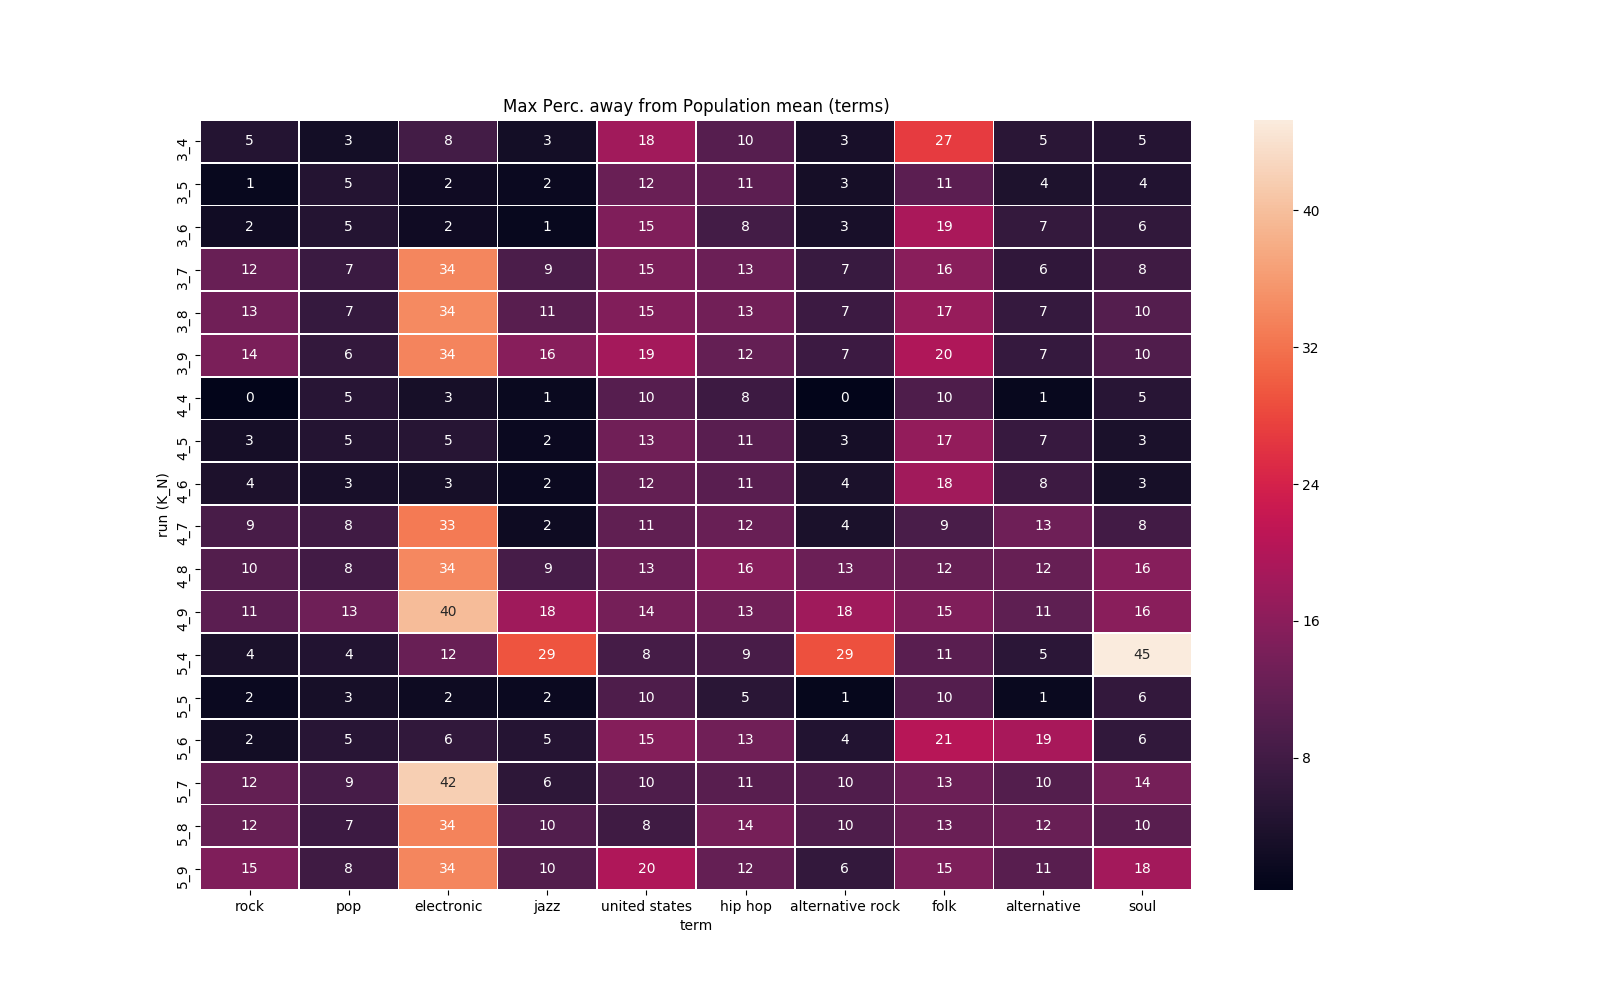
\includegraphics[width=1.2\textwidth]{perc_away_terms}
    \caption{Maximum difference between clusters and population}
    \label{fig:all}
\end{figure*}

We used a few different measures to determine how well clusters separated along genre, year, or artist.
All of the measures are summaries of a run's clusters, and compares against the entire dataset's counts.
We include the standard deviation of variable counts across each run's clusters,
the highest number of standard deviations away from the population count in a run,
and the highest difference in a run between a cluster's portion (in percentage) to the portion in the population.
These measures are all intended to detect if there are clusters that dramatically under or over represent a particular variable,
which would indicate the our clustering separates the variable well.

The results appear fairly noisy, without many discernible patterns.
Electronica music separates well when cluster sizes are $n=\{7,8,9\}$ (See figure~\ref{fig:all})
and 1940s music separates well when cluster sizes are $n=\{4,5,6\}$.

Artists terms in general seem to separate well (See Appendix), with the difference in percentages being
above 100\% of the population in most cases.
However, it should be noted that with artists,
the population frequency is very low (highest is about 0.1\%),
so even a cluster with 100 data points and a single occurrence of the artist will be 900\%
of the population frequency.
There are similar problems with the earlier decades being underrepresented, as can be seen above.

\subsection{K=5, N=4}

Across variables, when $k=5$ and $n=4$, clustering appears to separate better than normal.
So we will look at this cluster in a bit more depth.

\begin{figure*}[ht]
    \centering
    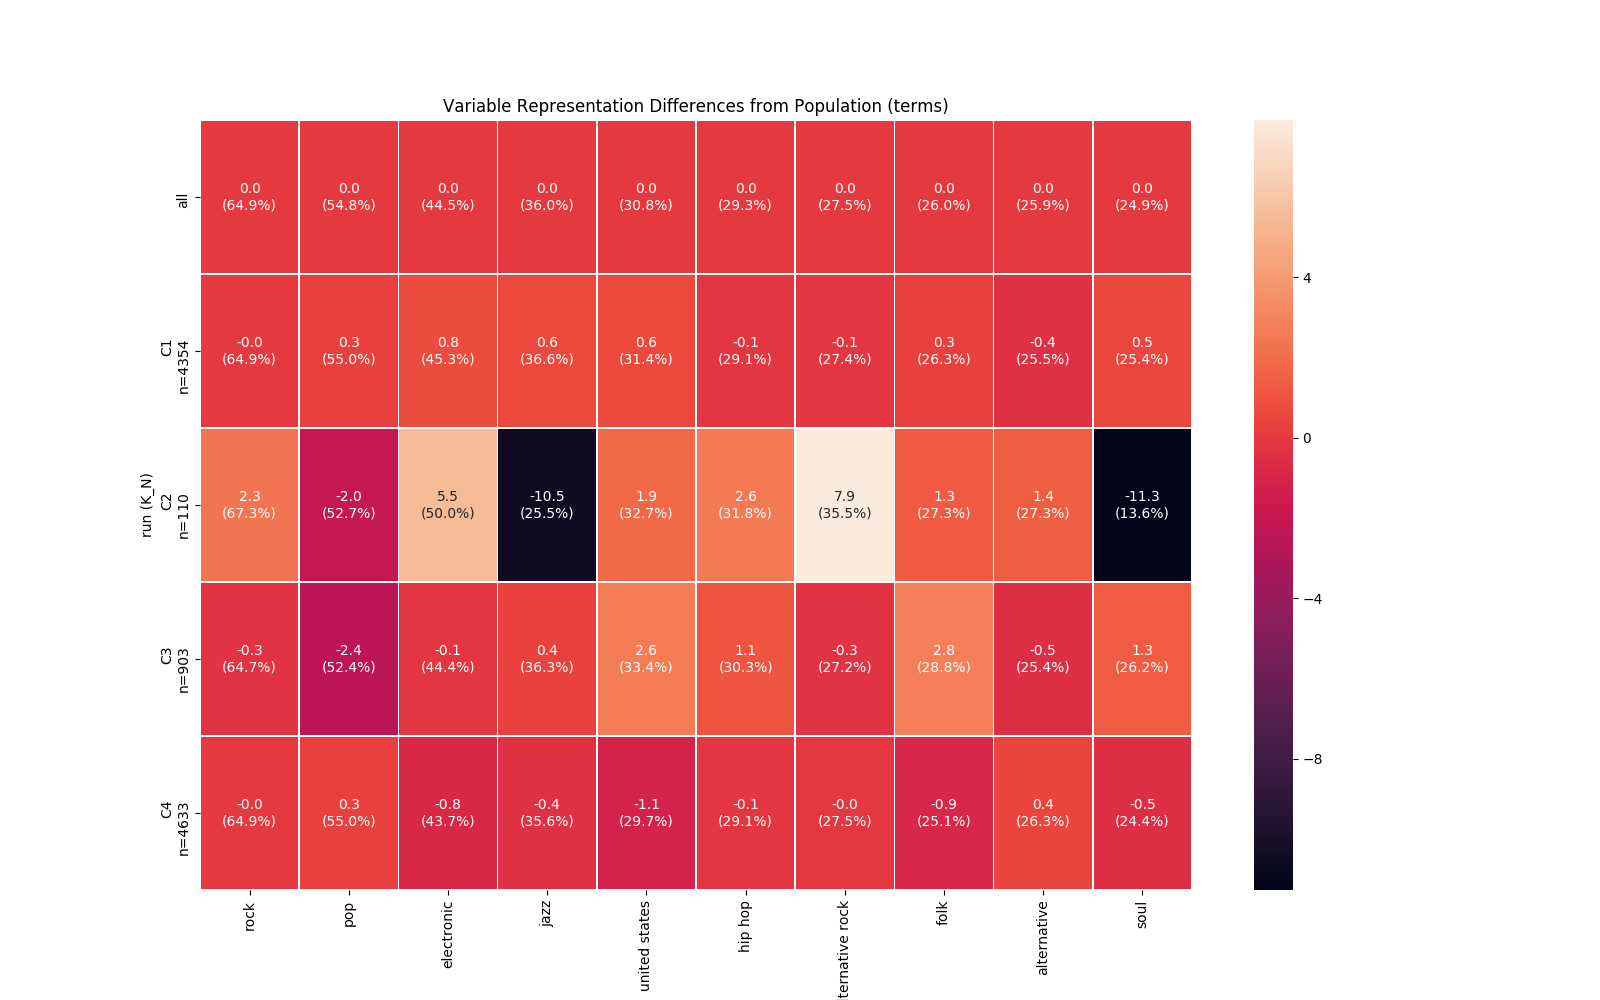
\includegraphics[width=1\textwidth]{terms_cluster}
    \caption{Population vs. Clustering with $k=5$ and $n=4$}
    \label{fig:cluster}
\end{figure*}

Figure~\ref{fig:cluster} show how the clusters are distributed for this run.
There are some stark outliers in how variables are represented between clusters,
such as Jazz, Alternative Rock, and soul in $C2$.
We think that much of this is due to sample size.
$C2$ only has 110 data points, which is much smaller than the other clusters.
The larger clusters are more uniformly distributed across all the variables,
which suggests that the abberations in $C2$ are due mainly to sample size.


    \section{Conclusion}
        It's hard to put a lot of work into an idea that generates no results.
It's helpful to think that we did not fail, we just found a way that doesn't work!
However, such a result does provide a lot of room for reflection, learning, and considerations on how to move forward.
We discuss below some of the broader ideas we learned.

\subsection{Going Forward}

Our approach to finding musical progenitors yielded no results,
but we have ideas for how we could potentially get our method to work in the future.
As mentioned above in the methods section,
on approach we could change is how we define the "oldest" songs in a cluster.
Tweaking that parameter would change how the centers are decided, and could potentially yield better results.

Another approach would be to use different variables.
We used every segmented variable available to us, but we left out the summarized variables.
With the high dimensionality of the segmented variables, this may not impact it too much.


\subsection{Data Cleaning Takes Time}

At least in our case, the most difficult part of our project was not implementing and extending an algorithm
from class, but in actually working with the data.
We spent a large chunk of our time, thought,
and energy on just getting the data into a format that we could use.
We had to consider how to deal with an unfamiliar format,
what form the data needed to be in to be able to use clustering,
how to deal with data of varying dimensions and length,
how to simplify and summarize certain types of data,
and how to process everything in an efficient manner.
Fortunately, our data was already fairly clean to begin with,
but even then it was a difficult task to clean.

Another aspect of data cleaning we didn't really consider until towards the end
was how to work with our own results.
Just having the data clustered isn't enough; we have to draw conclusions from those clusters.
We also spent a lot of time getting the results in a form that we could use to plot and analyze.

\subsection{Final Thoughts}

Working on an extension of a data mining method was a thought-provoking and intriguing project.
We had to consider properties of the Lloyds method,
and how our extension could potentially impact those properties.
We also had to consider how applying our method would work with our particular dataset.
In the end, it was a lot of work, but a lot more rewarding to apply to a project like this.


    \newpage
    \section{Distribution of Work}
        A.T is for Avram Twitchell, and A.D. is for Angel Dhungara

\begin{center}
\begin{tabular}{|l|r|r|r|} \hline
    Task                   & A.T.  & A.D.& Used in End? \\ \hline
    Raw H5 File Processing & x     &     & Yes          \\ 
    H5 to Matrix           & x     &     & Yes          \\
    Matrix to Counts       & x     &     & Yes          \\
    LSH                    & x     &     & No           \\
    Minhash                & x     &     & No           \\
    K++ Clustering         &       & x   & Yes          \\
    Gonzales Clustering    &       & x   & No           \\
    Lloyd Clustering       &       & x   & Yes          \\
    Hierarchical Clustering&       & x   & No           \\
    PCA Dim Reduction      &       & x   & No           \\
    Lloyd Extension        & x     &     & Yes          \\
    Run Experiment Script  & x     &     & Yes          \\
    Results Analyzer       & x     &     & Yes          \\
    Proposal               & x     & x   & Yes          \\
    Data Report            & x     &     & Yes          \\
    Intermediate Report    &       & x   & Yes          \\ 
    Final Report Plots     & x     & x   & Yes          \\
    Final Report-Intro     & x     &     & Yes          \\
    Final Report-Data      & x     &     & Yes          \\
    Final Report-Method    & x     &     & Yes          \\
    Final Report-Results   & x     &     & Yes          \\
    Final Report-Conclusion& x     & x   & Yes          \\ \hline
\end{tabular}
\end{center}

    \section{Appendix}
        \subsection{Standard Deviation Figures}
    \subsubsection{Genres}
        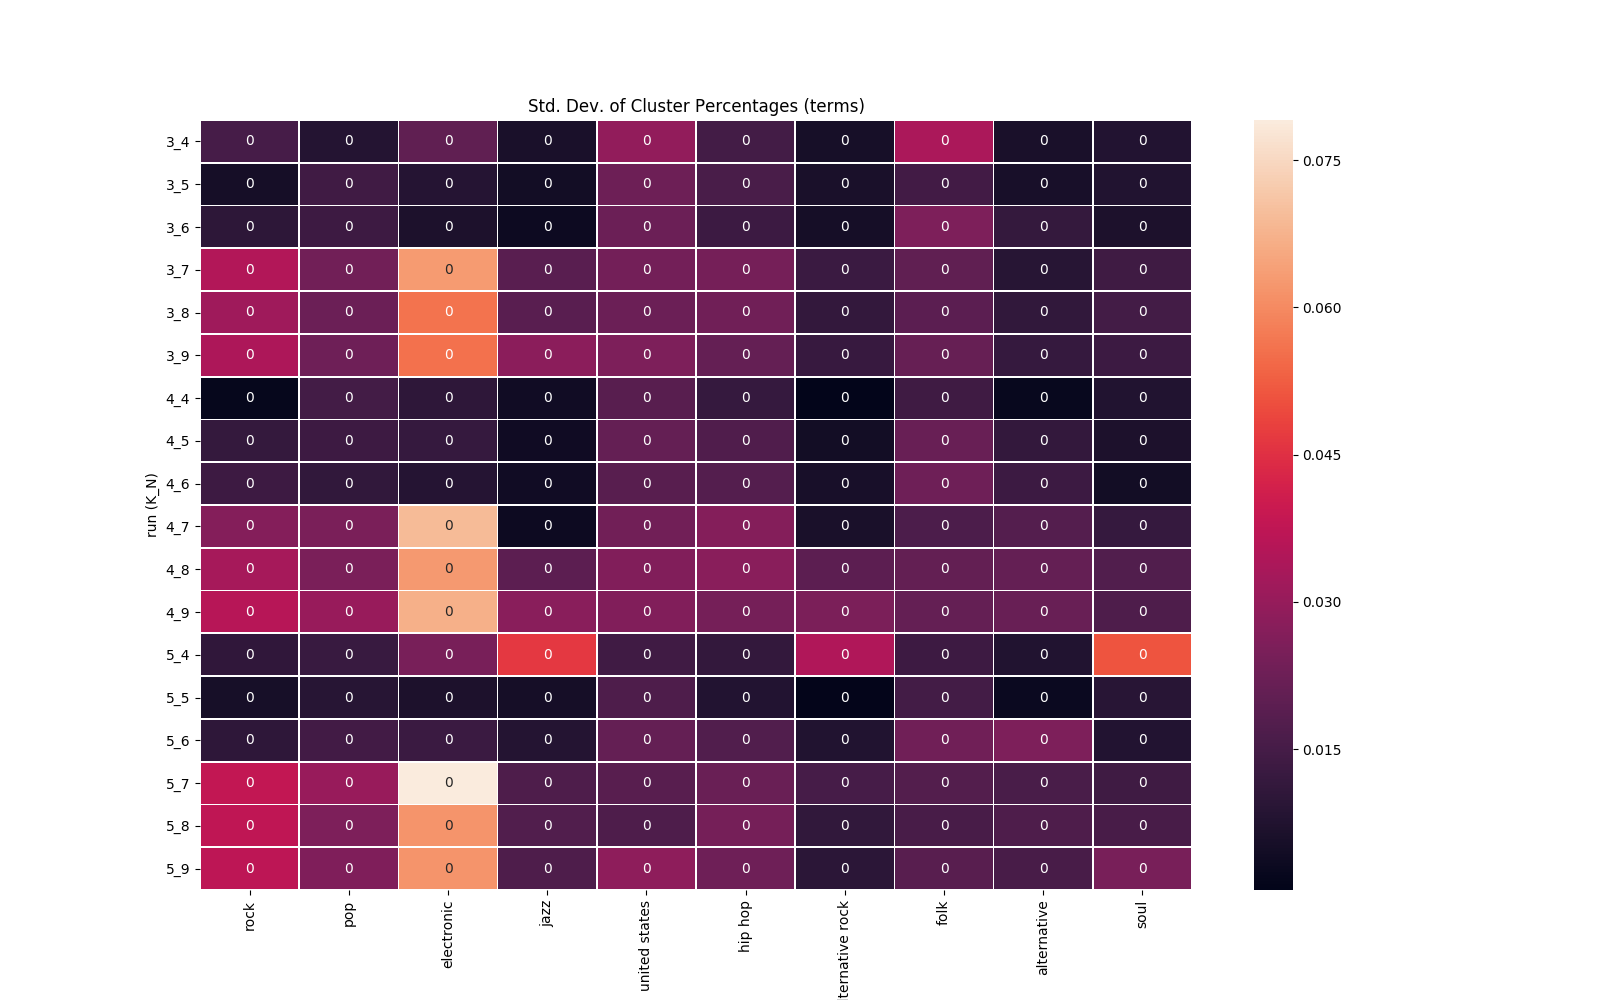
\includegraphics[width=1.2\textwidth]{sd_terms}
    \subsubsection{Decades}
        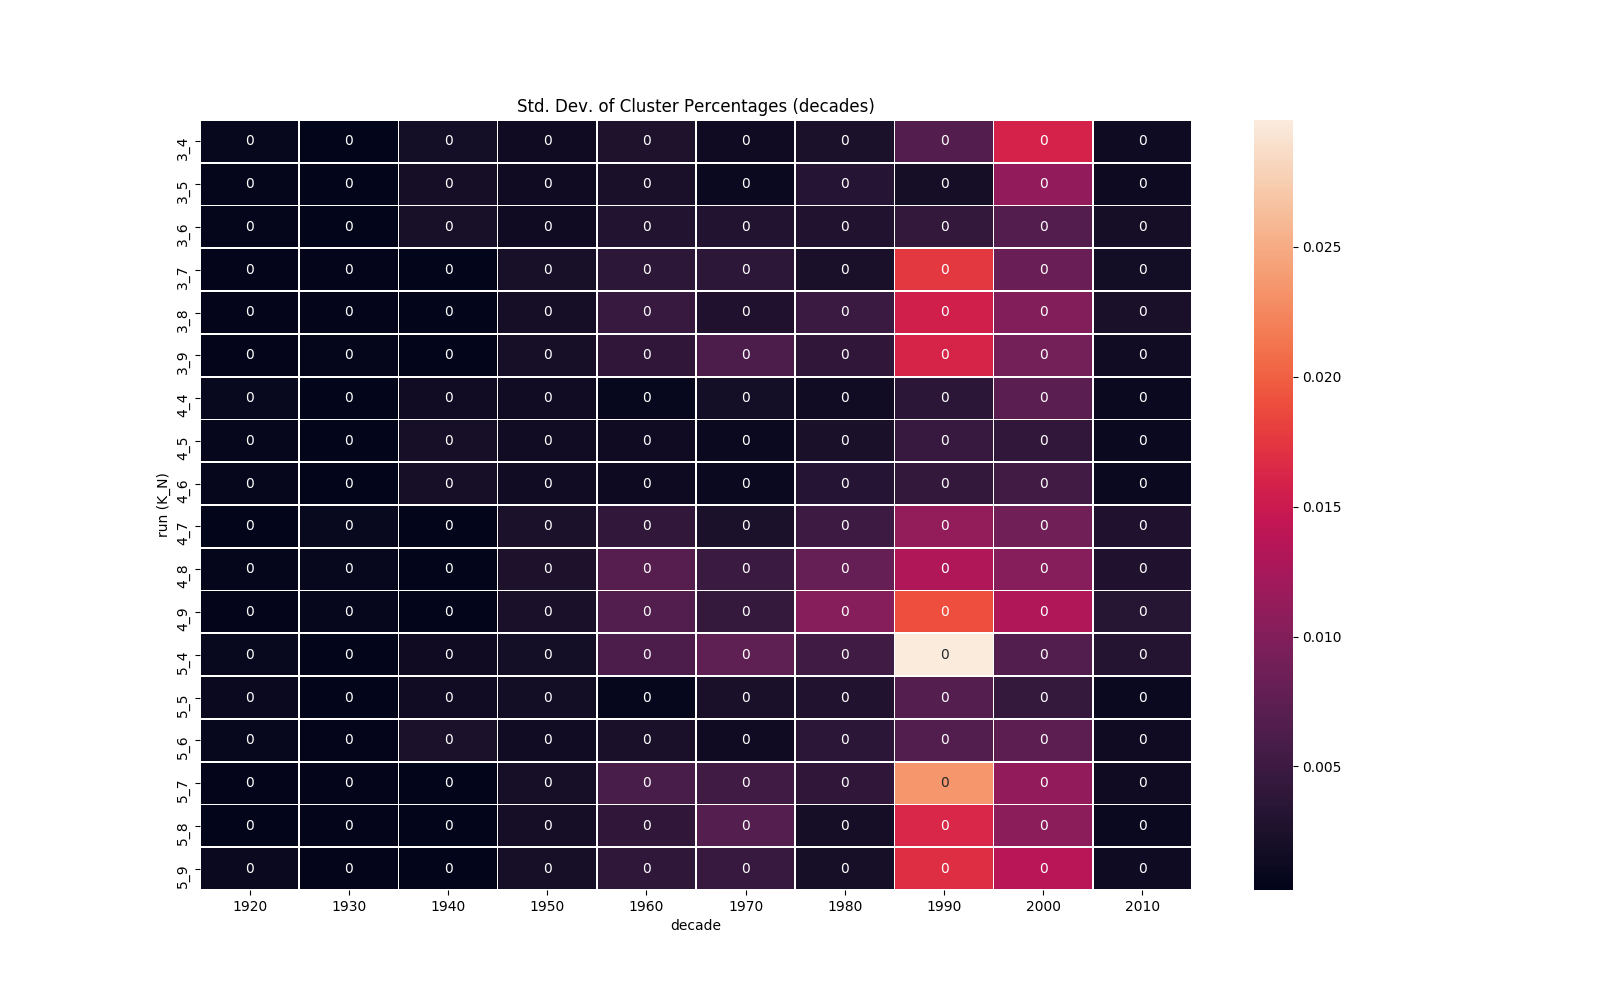
\includegraphics[width=1.2\textwidth]{sd_decades}
    \subsubsection{Artists}
        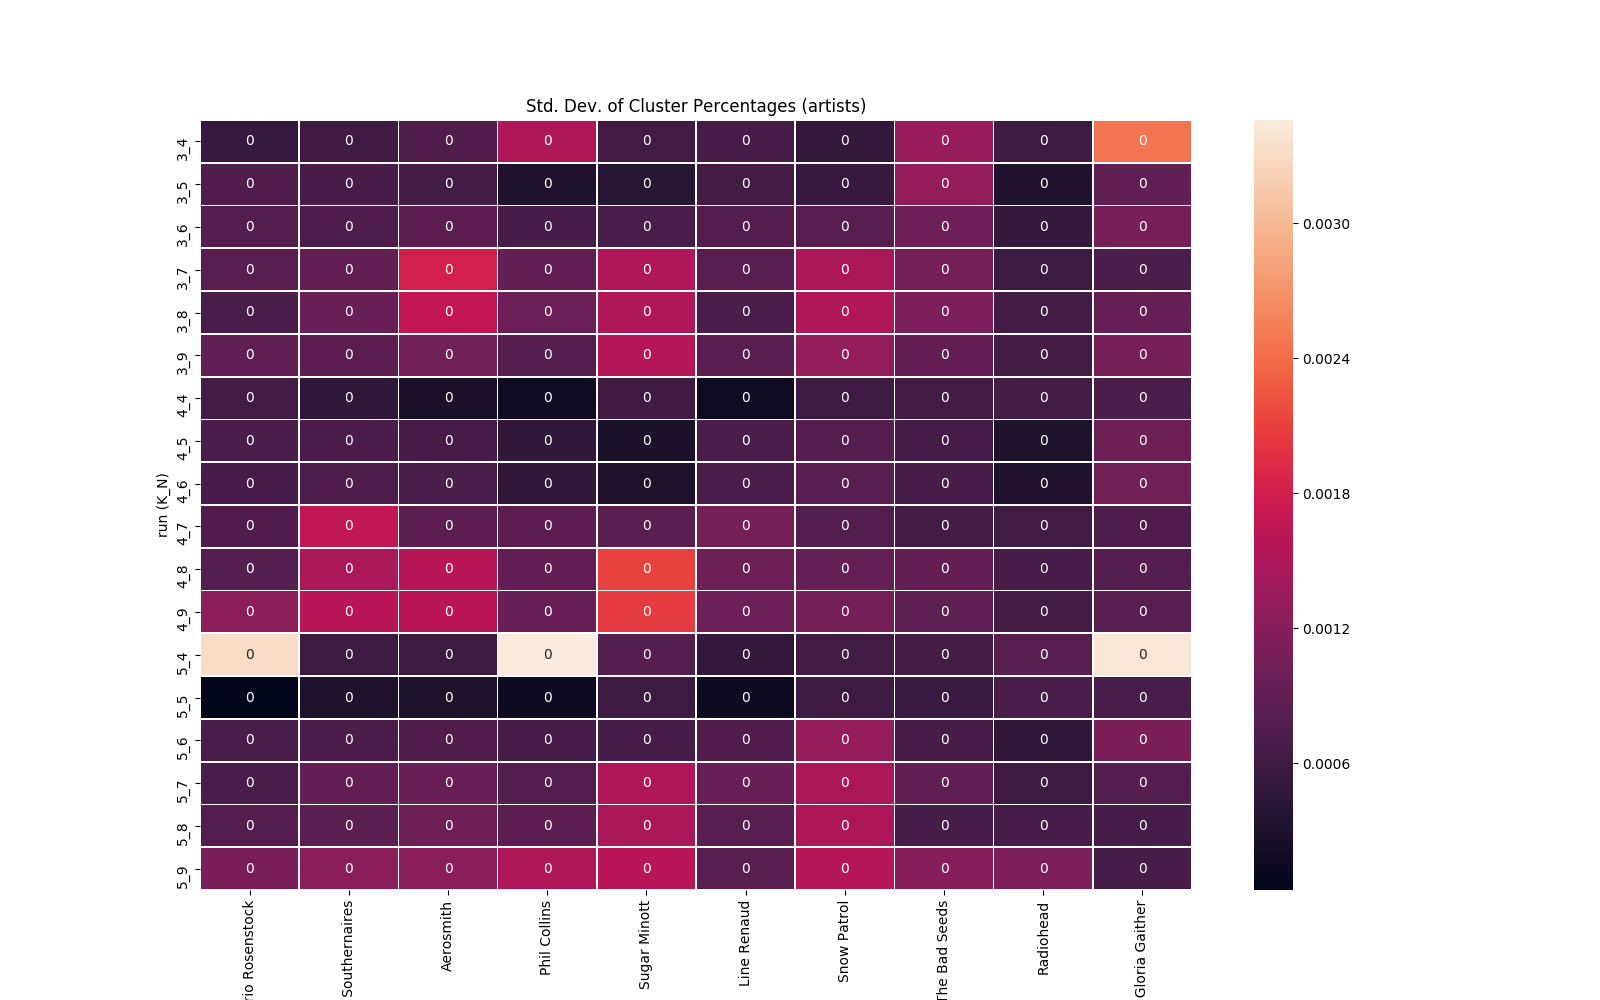
\includegraphics[width=1.2\textwidth]{sd_artists}

\subsection{Std. Dev. Away from Pop. Mean}
    \subsubsection{Genres}
        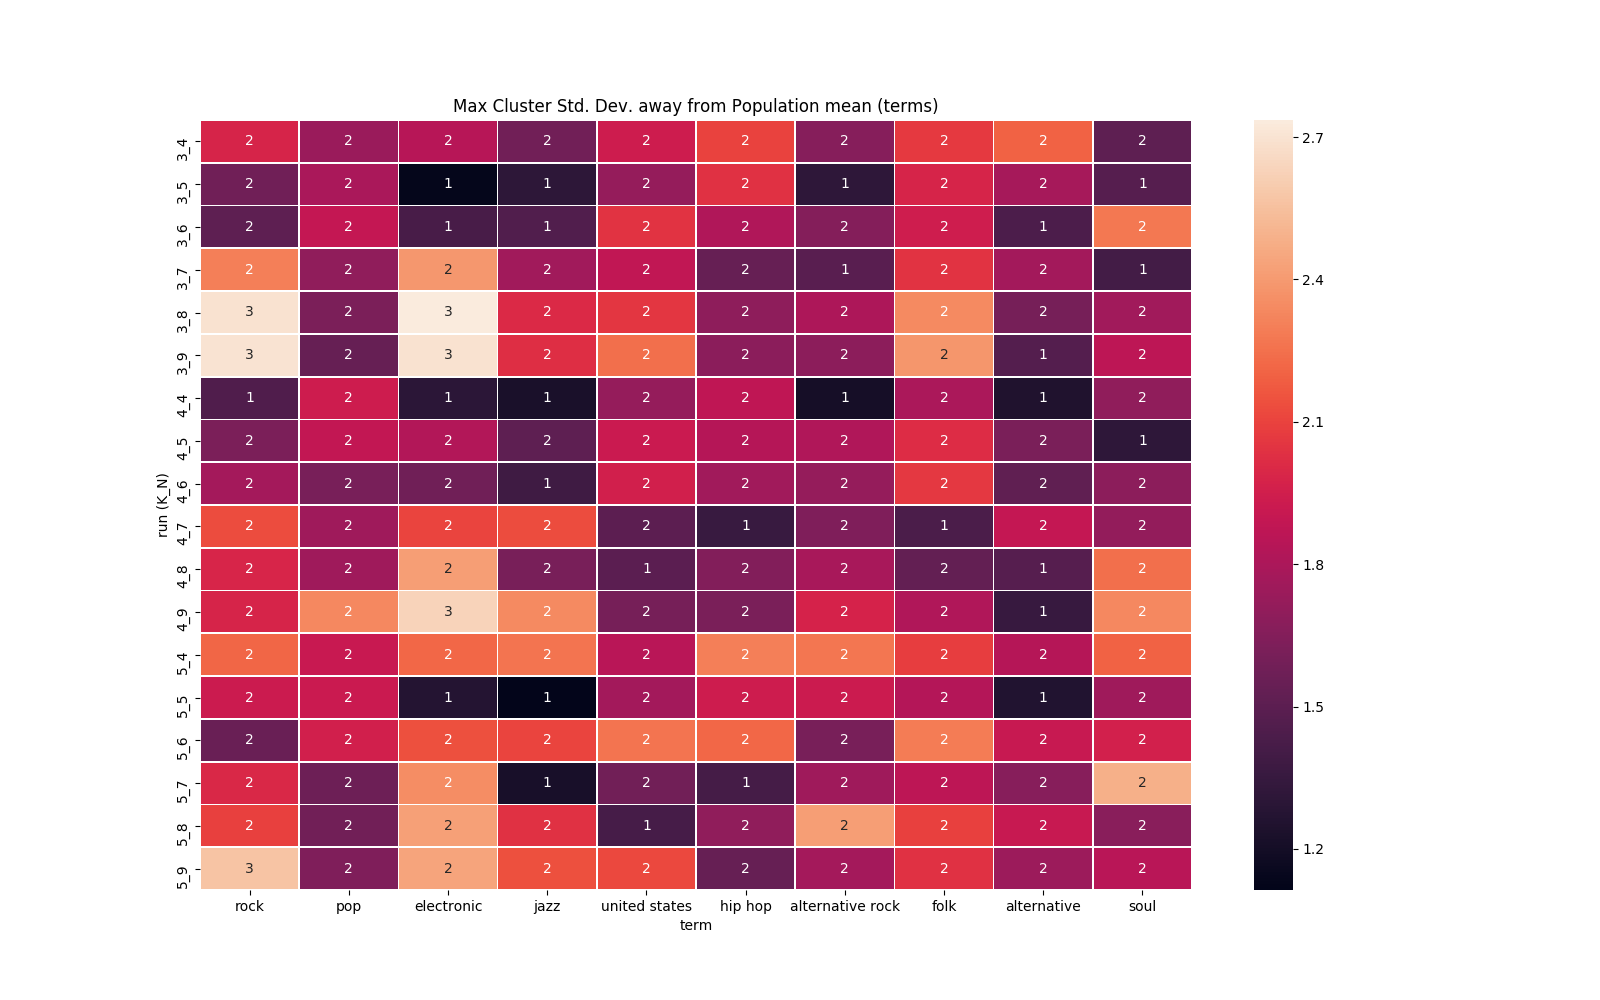
\includegraphics[width=1.2\textwidth]{sd_away_terms}
    \subsubsection{Decades}
        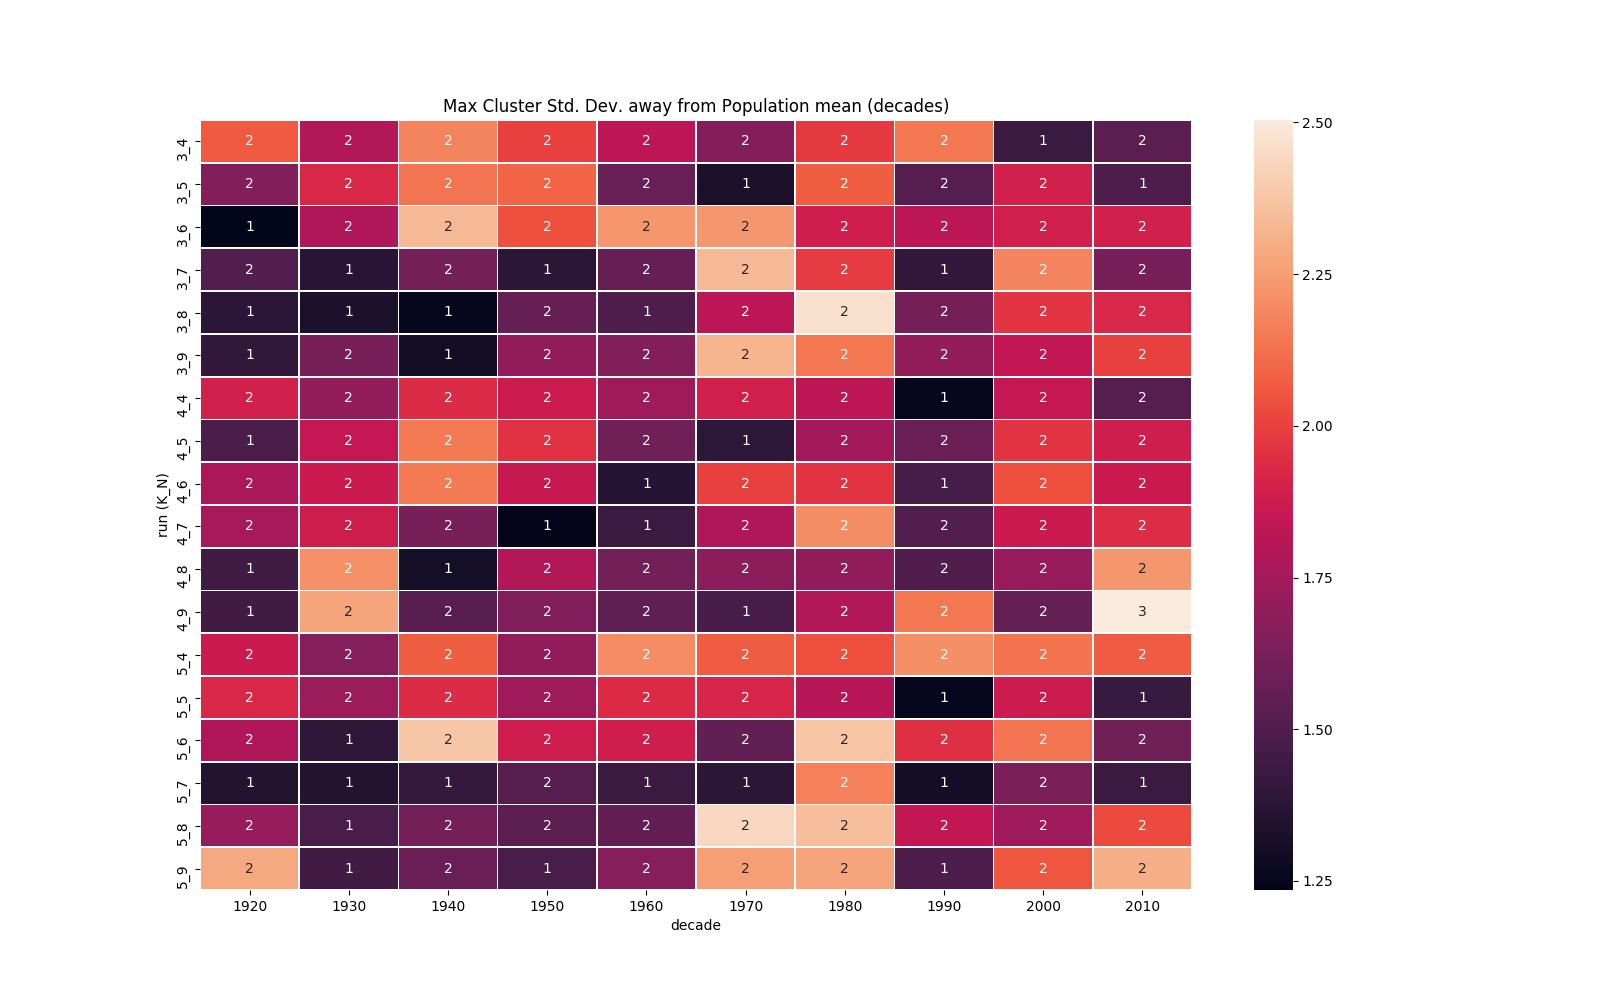
\includegraphics[width=1.2\textwidth]{sd_away_decades}
    \subsubsection{Artists}
        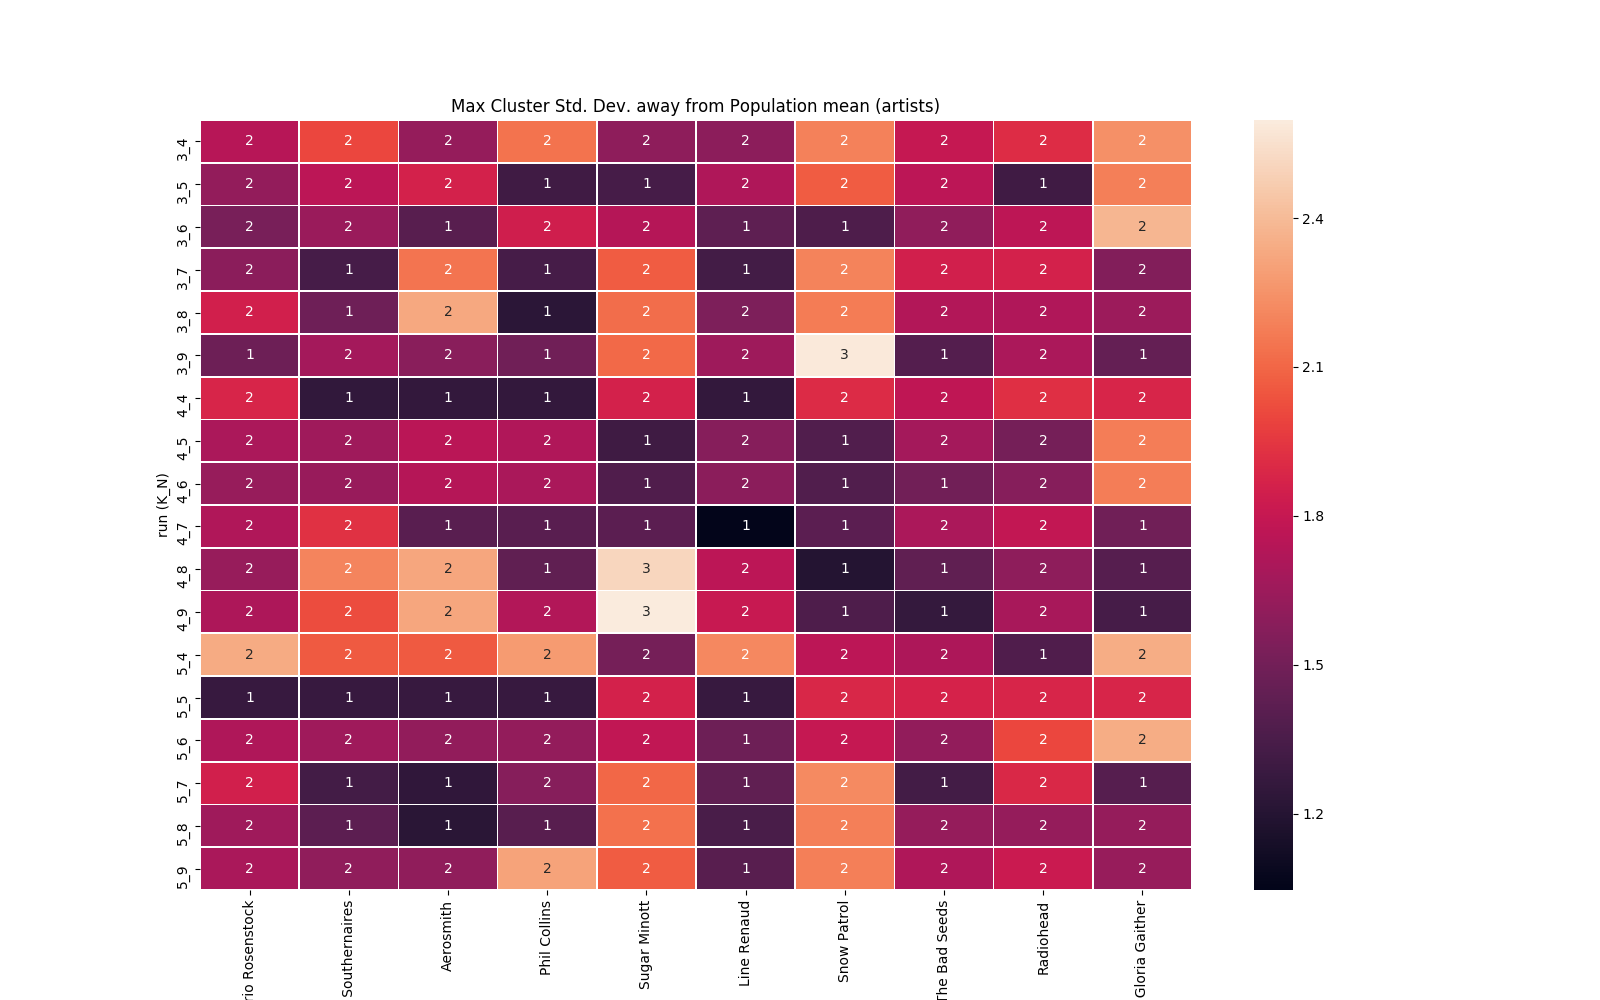
\includegraphics[width=1.2\textwidth]{sd_away_artists}

\subsection{Percentage Away from Pop. Mean}
    \subsubsection{Genres}
        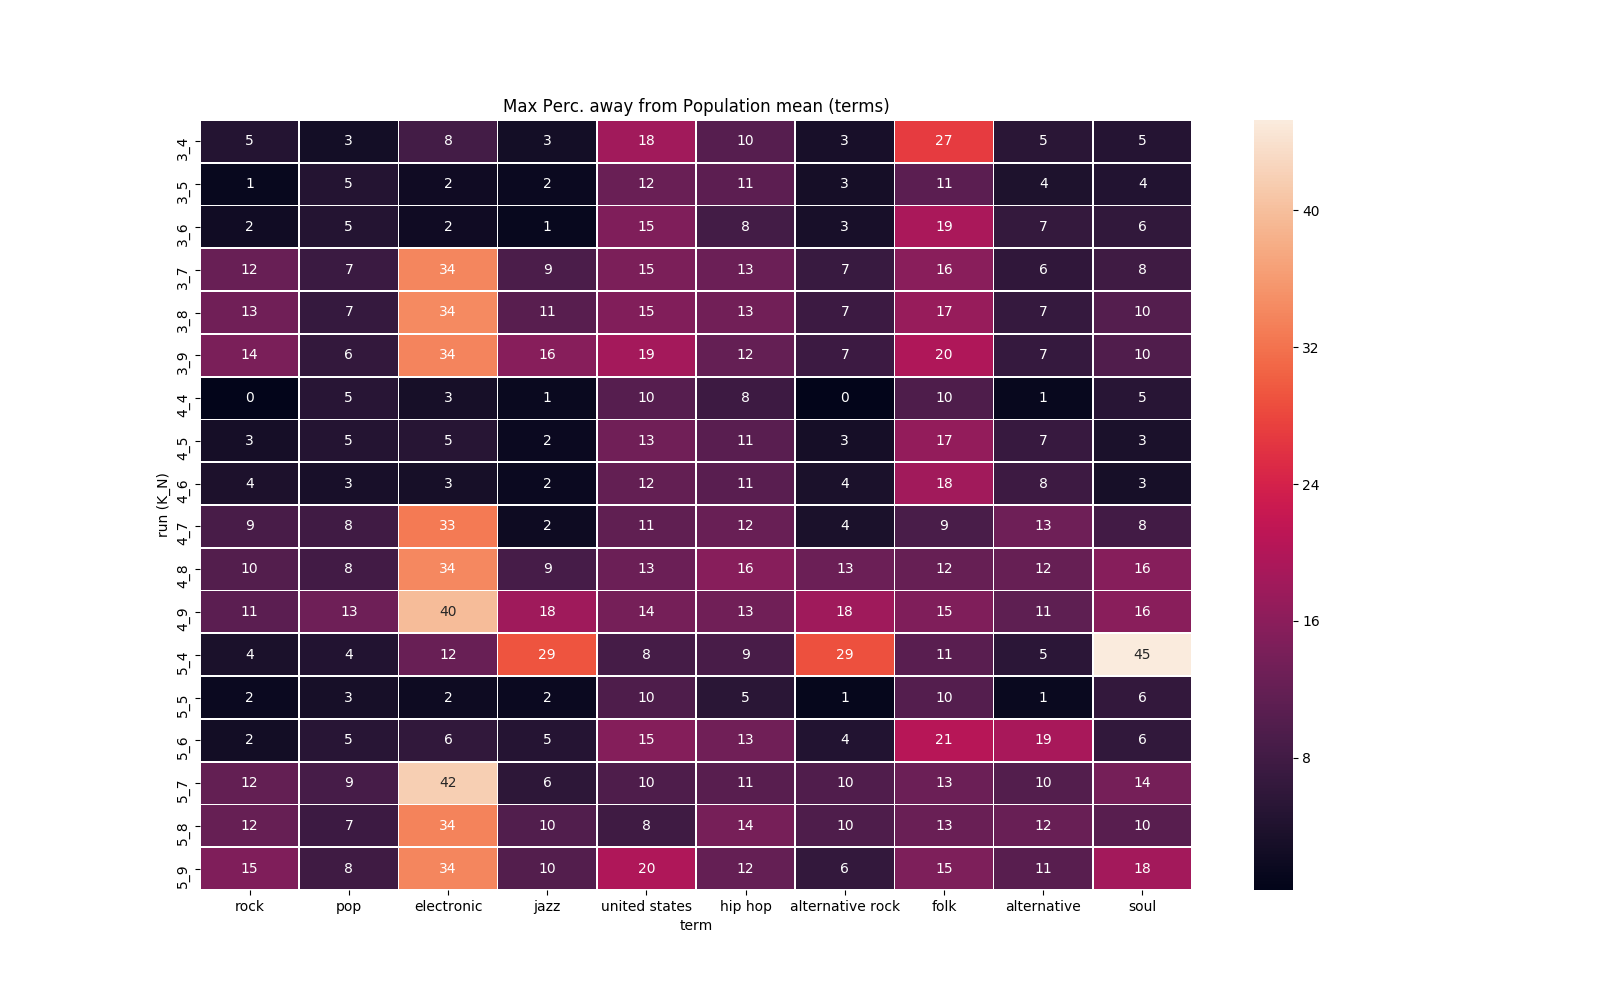
\includegraphics[width=1.2\textwidth]{perc_away_terms}
    \subsubsection{Decades}
        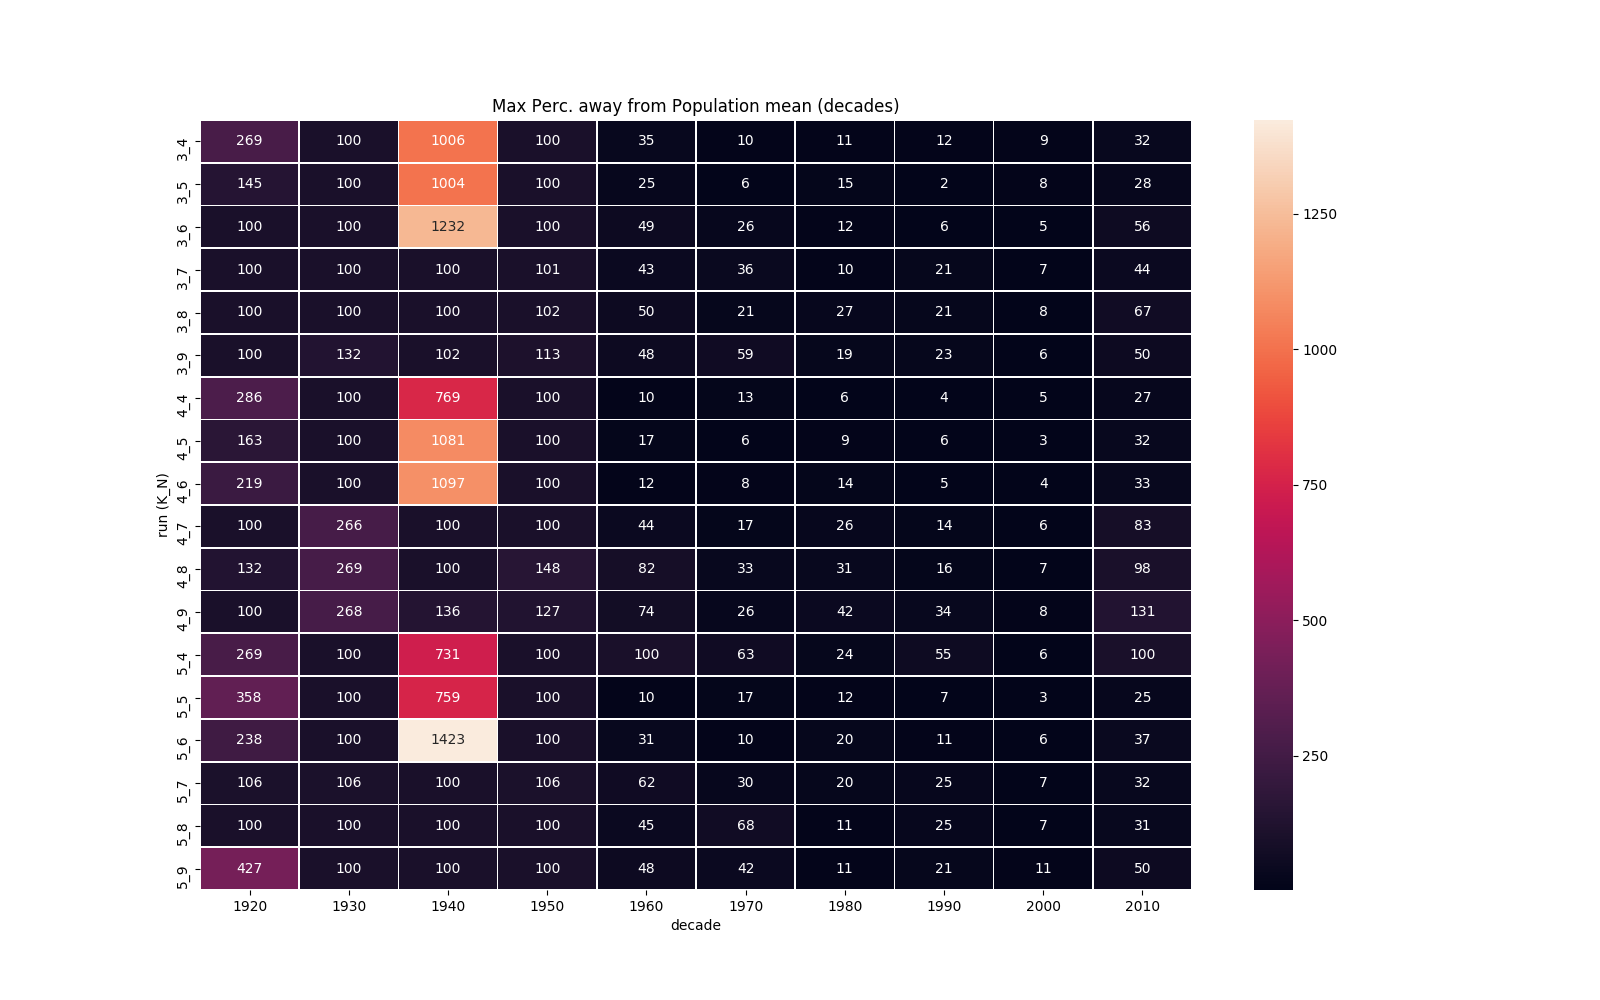
\includegraphics[width=1.2\textwidth]{perc_away_decades}
    \subsubsection{Artists}
        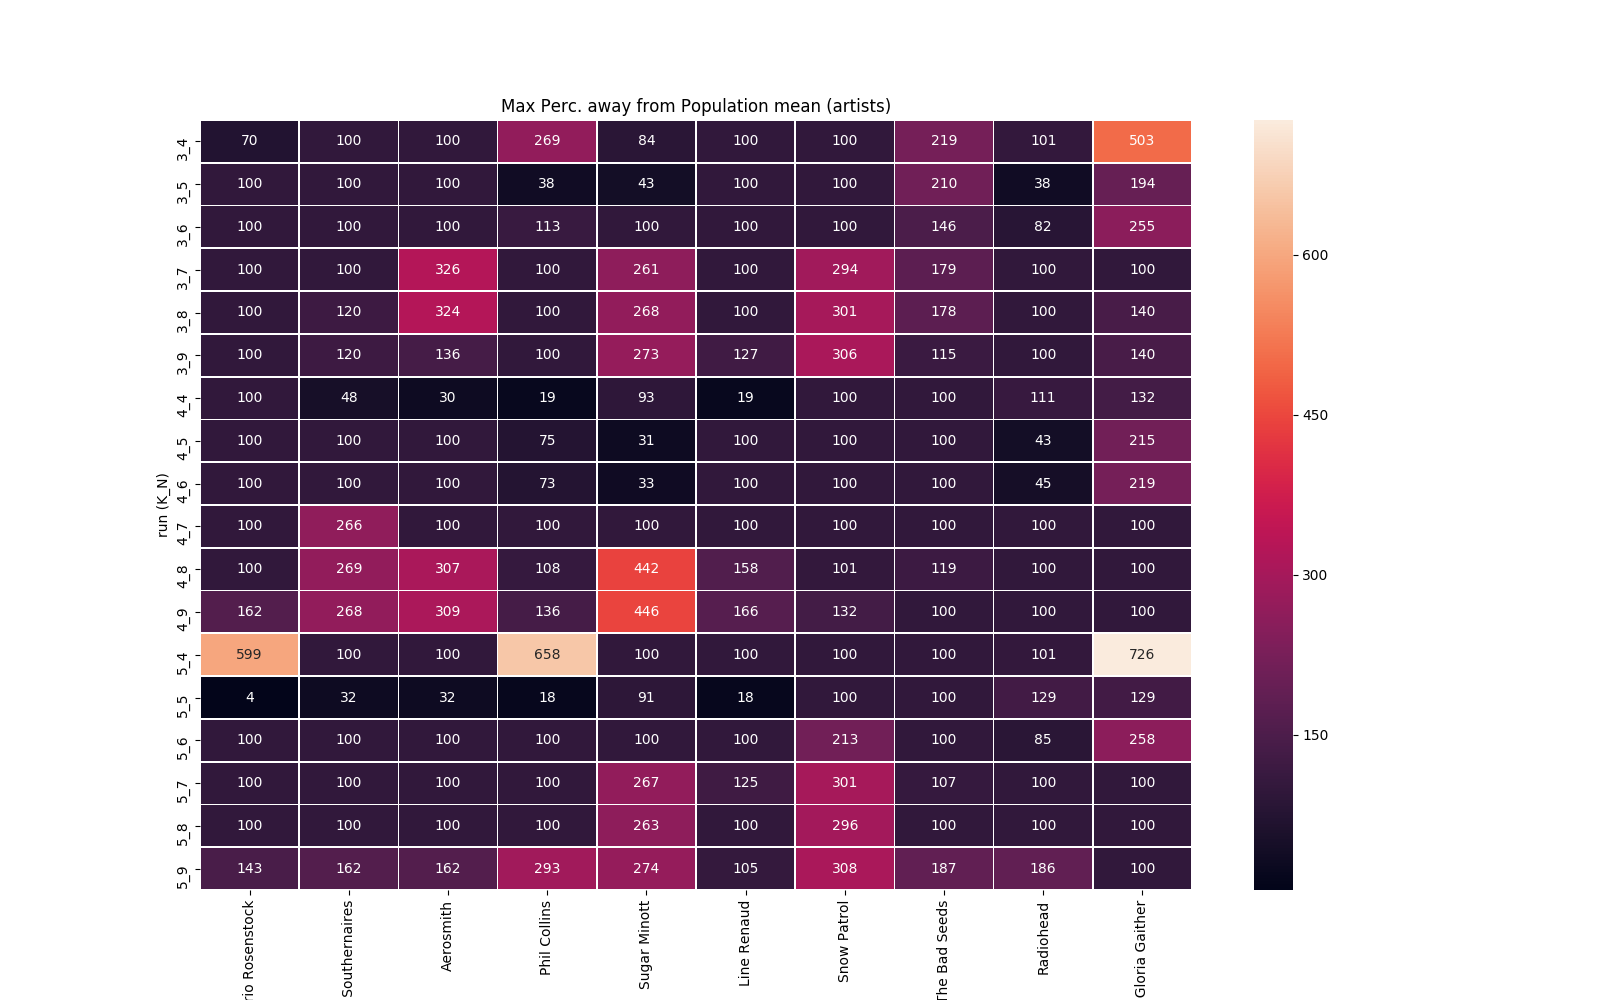
\includegraphics[width=1.2\textwidth]{perc_away_artists}

\subsection{Clustering with $k=5$, $n=4$}
    \subsubsection{Genres}
        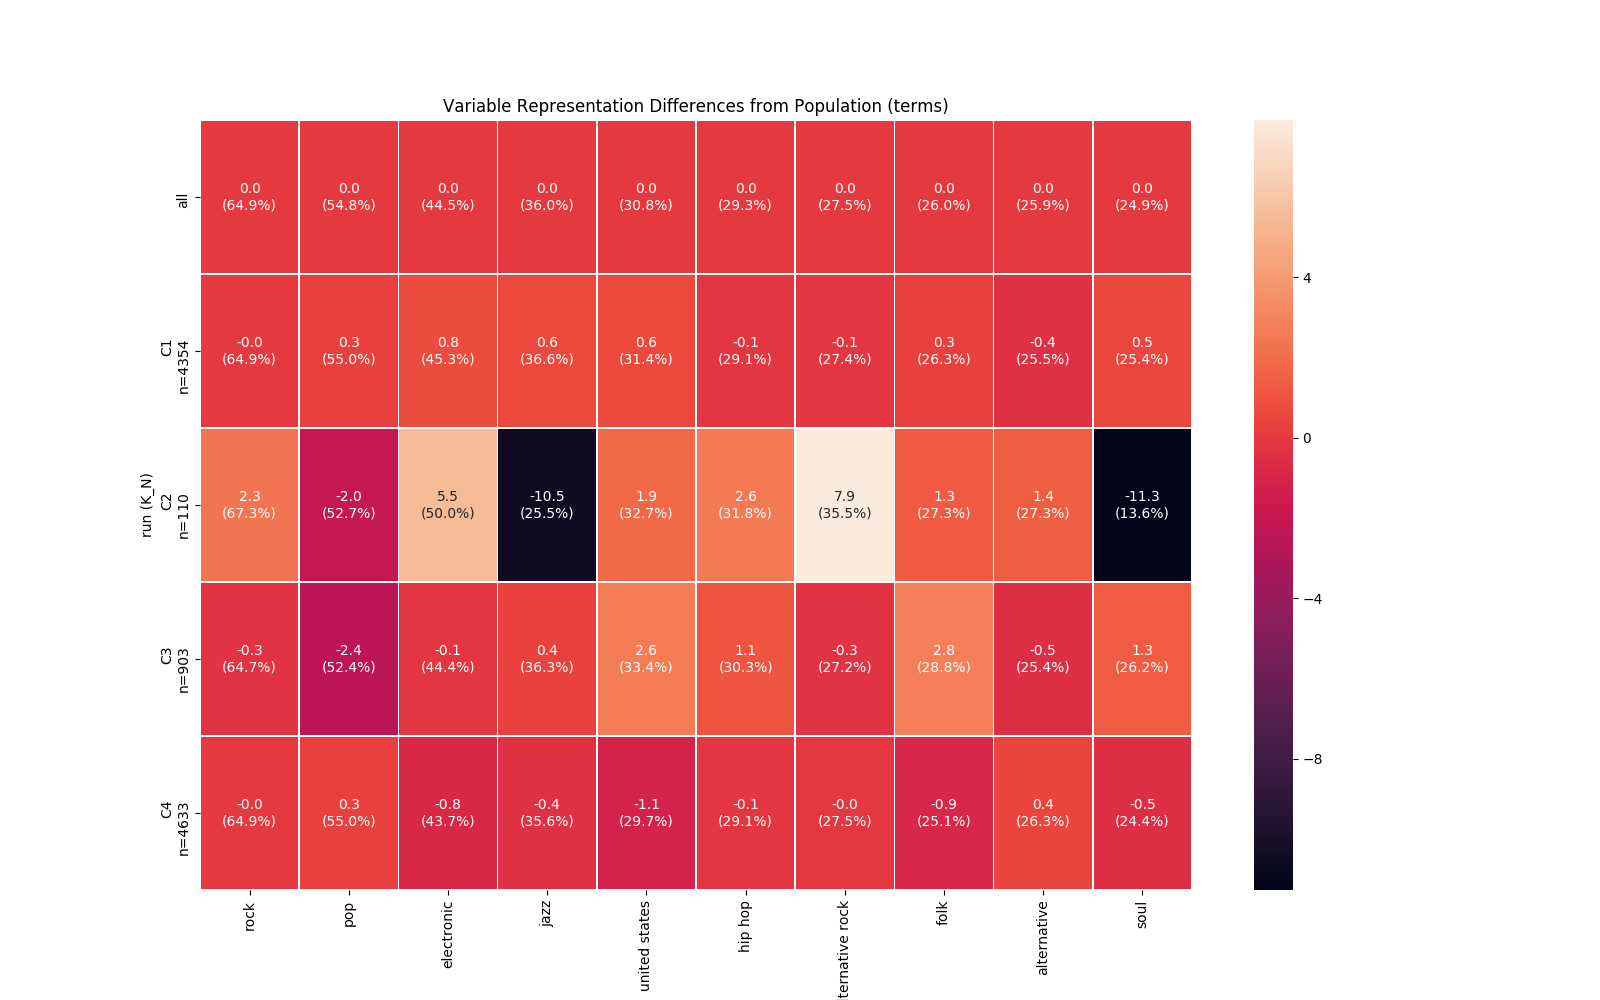
\includegraphics[width=1.2\textwidth]{terms_cluster}
    \subsubsection{Decades}
        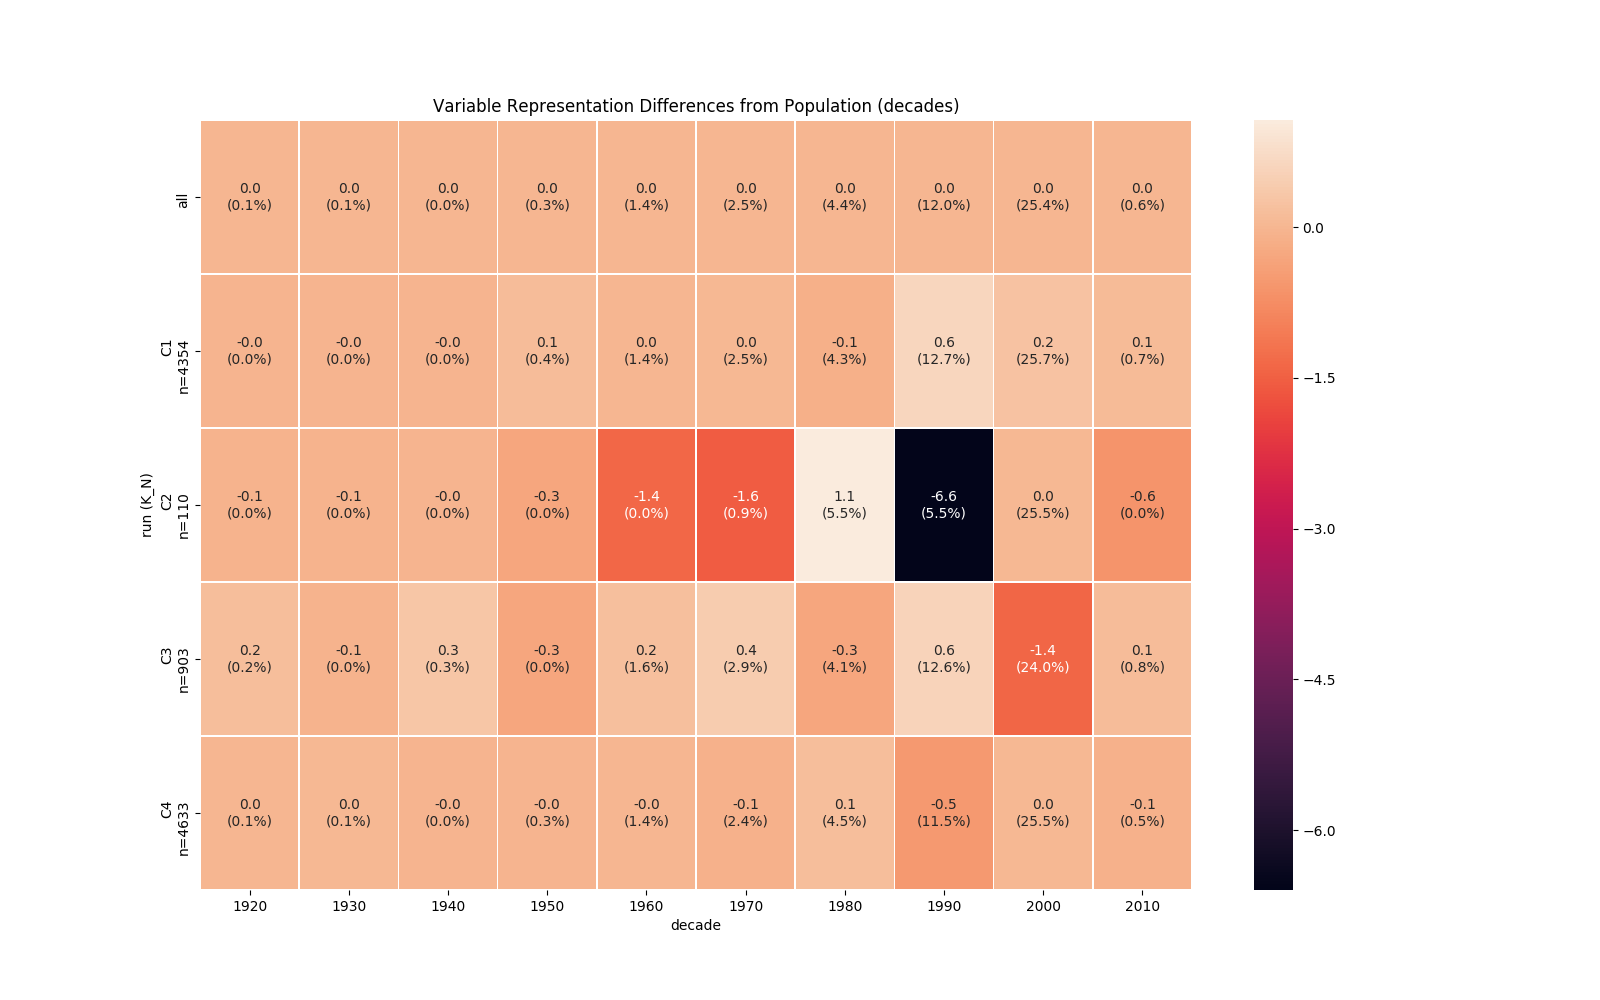
\includegraphics[width=1.2\textwidth]{decades_cluster}
    \subsubsection{Artists}
        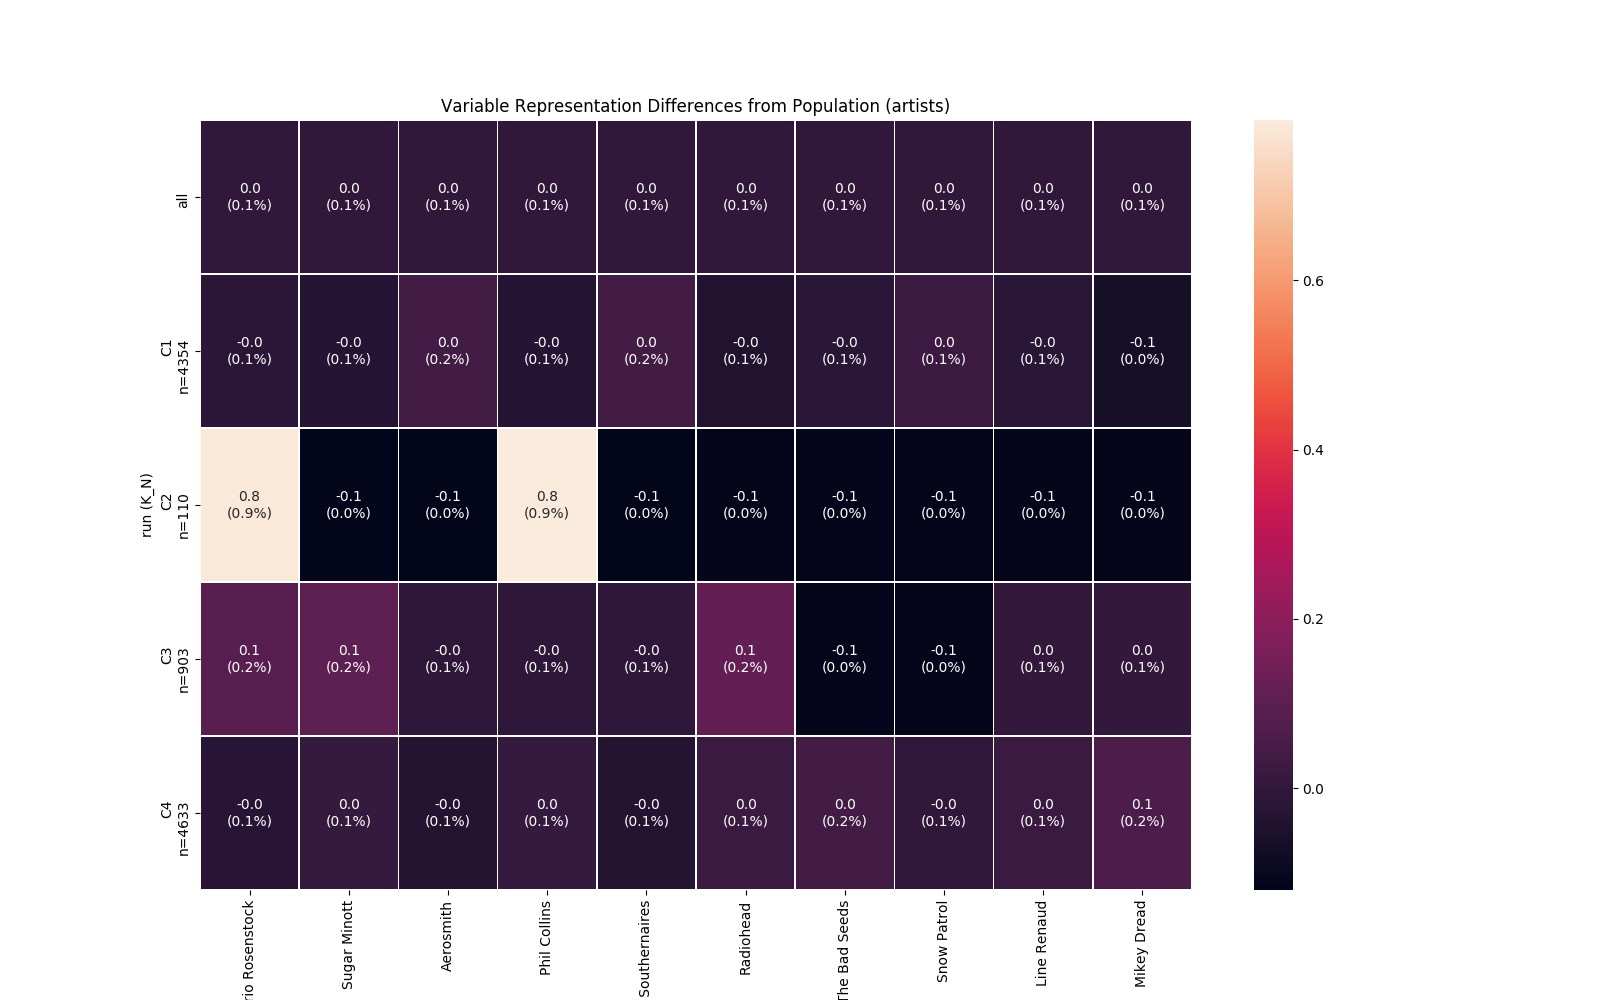
\includegraphics[width=1.2\textwidth]{artists_cluster}

   
\end{document}
